\chapter{Introduction}\label{chap:intro}

\section{Context}\label{sec:context}

\noindent Precise and dependable systems have become essential in an era where enterprises are driven toward more accuracy and efficiency by technology breakthroughs. The broadcast and entertainment industries have experienced significant expansion among these sectors due to the growing demand for immersive visual experiences enabled by \ac{AR} and \ac{VR} technologies. These innovations are transforming the way people consume material by providing them with interactive and captivating experiences. WTVision, a top business that specializes in real-time graphics and augmented reality solutions for many industries, is at the vanguard of this transformation.


\noindent The dynamic, aesthetically captivating settings that WTVision's technology helps creating for live broadcasts, sporting events, and virtual productions are essential. Achieving the desired level of realism that viewers anticipate requires a smooth transition between \ac{CGI} and real-world sights. But there are several obstacles in the way of reaching this level of visual accuracy, especially when it comes to camera lens calibration, which is essential to collecting real-world situations and matching them with virtual features.


\noindent To reduce image distortion, a frequent problem brought on by the physical characteristics of lenses, lens calibration is essential. In AR and VR settings, distortion can cause errors that impair the user experience. This difficulty is increased in apps that use varying zoom and focus settings since each one needs to be precisely calibrated in order to guarantee proper alignment of the virtual and real elements. At the moment, the labor- and time-intensive process of calibrating camera lenses takes four to eight hours and involves manual adjustments. The repetitive nature of the work and human mistake both make the process even more inefficient.


\noindent The limits of manual calibration approaches become more evident as the demand for AR and VR applications grows, especially in live broadcasts and virtual events. An automated solution that can speed up the calibration process and increase accuracy while decreasing time is desperately needed as a result of this. In light of this, the project's goal is to create a lens calibration algorithm that makes use of cutting-edge tools like image analysis and machine learning. The aim is to achieve maximum precision while radically reducing the time needed for the calibration process through automation and optimization.


\noindent The suggested method has the ability to greatly increase workflow efficiency in sectors that depend on accuratly determined camera lens distortion coefficients by resolving these issues. WTVision is ideally positioned to spearhead this endeavor and shape the future of immersive broadcast experiences because to its experience with real-time graphics and augmented reality technologies. If this effort is successful, it could improve the visual quality of AR and VR material and establish new guidelines for lens calibration procedures in a variety of businesses.
\section{wTVision}\label{sec:wTVision}


\noindent wTVision is a company \cite{wtvision} specialized in creating integrated broadcasting solutions, focusing on software development, graphics design and live operations.
\noindent Founded in 2001 and part of the Mediapro Group, wTVision has become a significant player in the broadcasting industry. The company provides a wide range of services, including real-time graphics, playout automation, augmented reality, virtual productions, and data distribution, serving live broadcasts, sports events, election coverage, entertainment shows, and news programs.


\noindent The company became one of the main real-time on-air graphics and playout automation providers due to its flexible solutions that can be integrated with multiple major graphics engines on the market. From small one time broadcasts to some of the most important competitions, wTVision takes part in more than 7 000 broadcasts annually and has experience in more than 120 countries. 
wTVision has hundreds of specialists around the globe and offices in Portugal, Spain, Belgium, Brazil, Bolivia, United Arab Emirates, India and USA.

\noindent Given that the sports industry is a primary focus for the company, and football is the dominant market in Portugal and many other countries, artificial intelligence and computer vision present a wide range of new opportunities to be explored. As a result, this topic has been increasingly investigated by researches over the past years. 


\section{Problem Definition and Internship Goals}\label{sec:intern_goals}

\noindent This section presents a clear description of the current problem. This section will use the following fundamental concepts: \textbf{Augmented Reality \ac{AR}}, \textbf{lens distortion} and the \textbf{$R^3$ software}. A detailed explanation of each can be found in chapter \ref{chap:state_art}.

\noindent wTVision developed the \( R^3 \) software for creating virtual environments and integrating virtual objects into real scenes. This software enables augmented reality experiences by seamlessly introducing virtual elements into live footage. However, it does not account for lens distortion, meaning virtual objects remain undistorted while the real scene may exhibit natural optical warping. The challenge of this project is not to correct lens distortion but to accurately replicate it within virtual environments, ensuring a more realistic and cohesive augmented reality experience.

\noindent The limitations of the $R^3$ software, including its reliance on operator expertise, time-intensive calibration process, and lack of automation for dynamic zoom and focus adjustments, underscore the need for a more efficient solution.

\noindent This thesis aims to improve the calibration process by:
\begin{itemize}
    \item Reducing reliance on operator expertise.
    \item Automating the process to decrease calibration time.
\end{itemize}

\subsection{Current Solution} \label{sec:current_solution}

\noindent This section focuses on wTVision’s current solution for calibrating a virtual environment, which
involves using the $R^3$
software to distort the virtual environment to match the distortion observed
in the real world.

\noindent While this approach is effective, the quality of the calibration—and, consequently, the realism of the virtual overlays—relies heavily on the calibration operator’s experience and expertise. Additionally, it is a time-consuming process, typically taking between 4 to 6 hours.

\subsubsection*{Detailed Calibration Process}

\noindent The calibration process involves determining the calibration coefficients in the following order:

\begin{itemize}
    \item Center-shift
    \item Field of View
    \item \( k_1 \) (radial distortion)
    \item \( k_2 \) (radial distortion at the edges)
    \item Nodal Point
\end{itemize}

\subsubsection*{Calibration Preparation}

\noindent Before starting the calibration process, the dimensions and coordinates of a real object on a real scene must be defined and provided to the $R^3$ software. This step can be completed either before or after the center-shift calibration. The following steps outline the calibration process for each coefficient:

\begin{enumerate}
    \item \textbf{Center-Shift:}  Align the virtual object with the real object at the center of the image.
    Adjust the central-shift coefficient until they match at minimum and maximum zoom levels.
    Intermediate values are interpolated.
    Figure \ref{fig:Cone} illustrates the current process for calibrating this coefficient. First, a real-world
    image with a reference point is required; typically, a phone light is used to produce the white circle in the
    image shown at the top of Figure \ref{fig:Cone}. Next, a cone is introduced. This cone does not
    need any specific characteristics other than having a pointy end. The center-shift is then
    adjusted, as depicted, until the pointy end of the cone aligns with the center of the white
    circle of light. After achieving this alignment, zoom in and verify that the pointy end
    remains at the center of the circle of light. If not, readjust the center-shift accordingly.

    Figure \ref{fig:Cone} illustrates the current process for calibrating this coefficient. First, a real-world image with a reference point is required; typically, a phone light is used to produce the image shown at the top of Figure \ref{fig:Cone}. Next, a cone is introduced. This cone does not need any specific characteristics other than having a pointy end. The center-shift is then adjusted, as depicted, until the pointy end of the cone aligns with the center of the white circle of light. After achieving this alignment, zoom in and verify that the pointy end remains at the center of the circle of light. If not, readjust the center-shift accordingly.
    
    \begin{figure}[h]
    \centering
    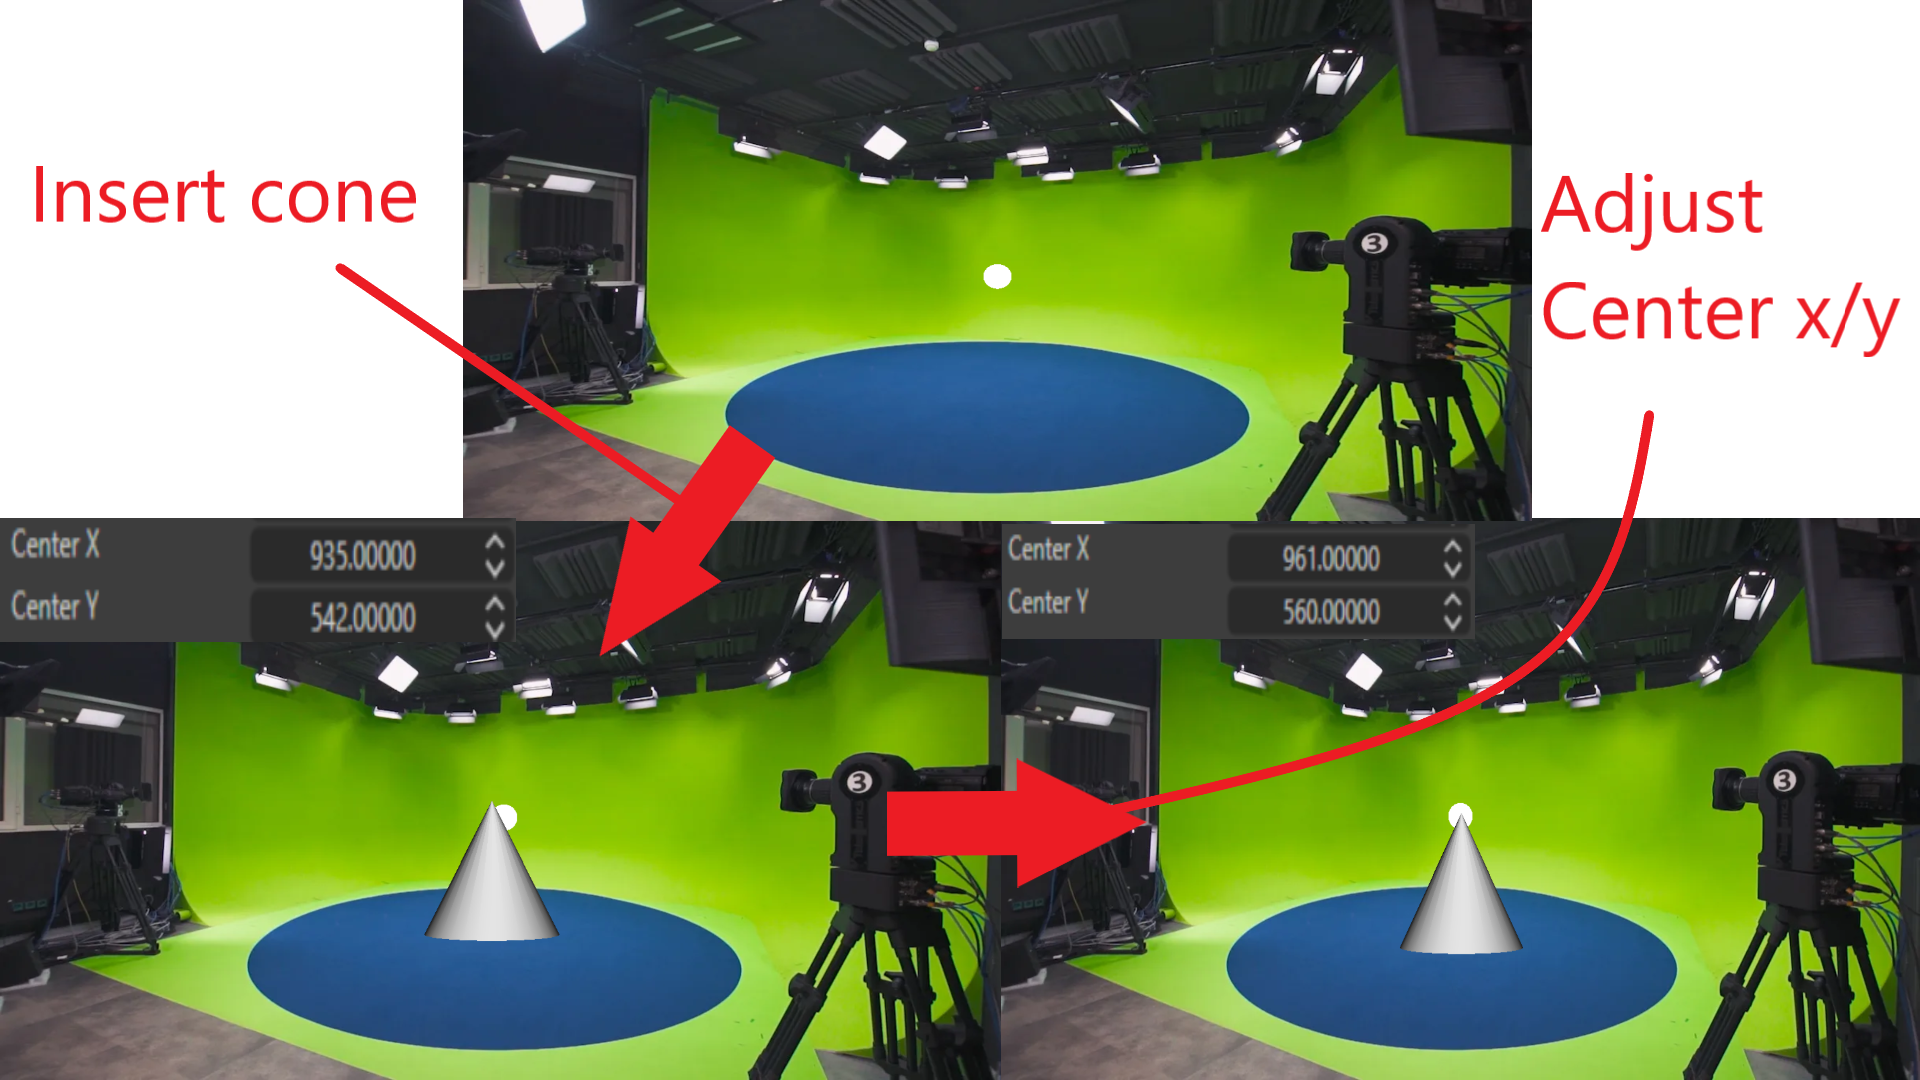
\includegraphics[width=\textwidth]{Images/01intro/Cone.png}
    \caption{Center shift calibration procedure example}
    \label{fig:Cone}
    \end{figure}
    
    
    
    \item \textbf{Field of View:} Move the real object (red square) off-center, then align the virtual object with the real object. Repeat this process for seven zoom levels to capture variations in distortion. Figure \ref{fig:FoV_pro} illustrates the calibration procedure for a FoV.

    \begin{figure}[h]
    \centering
    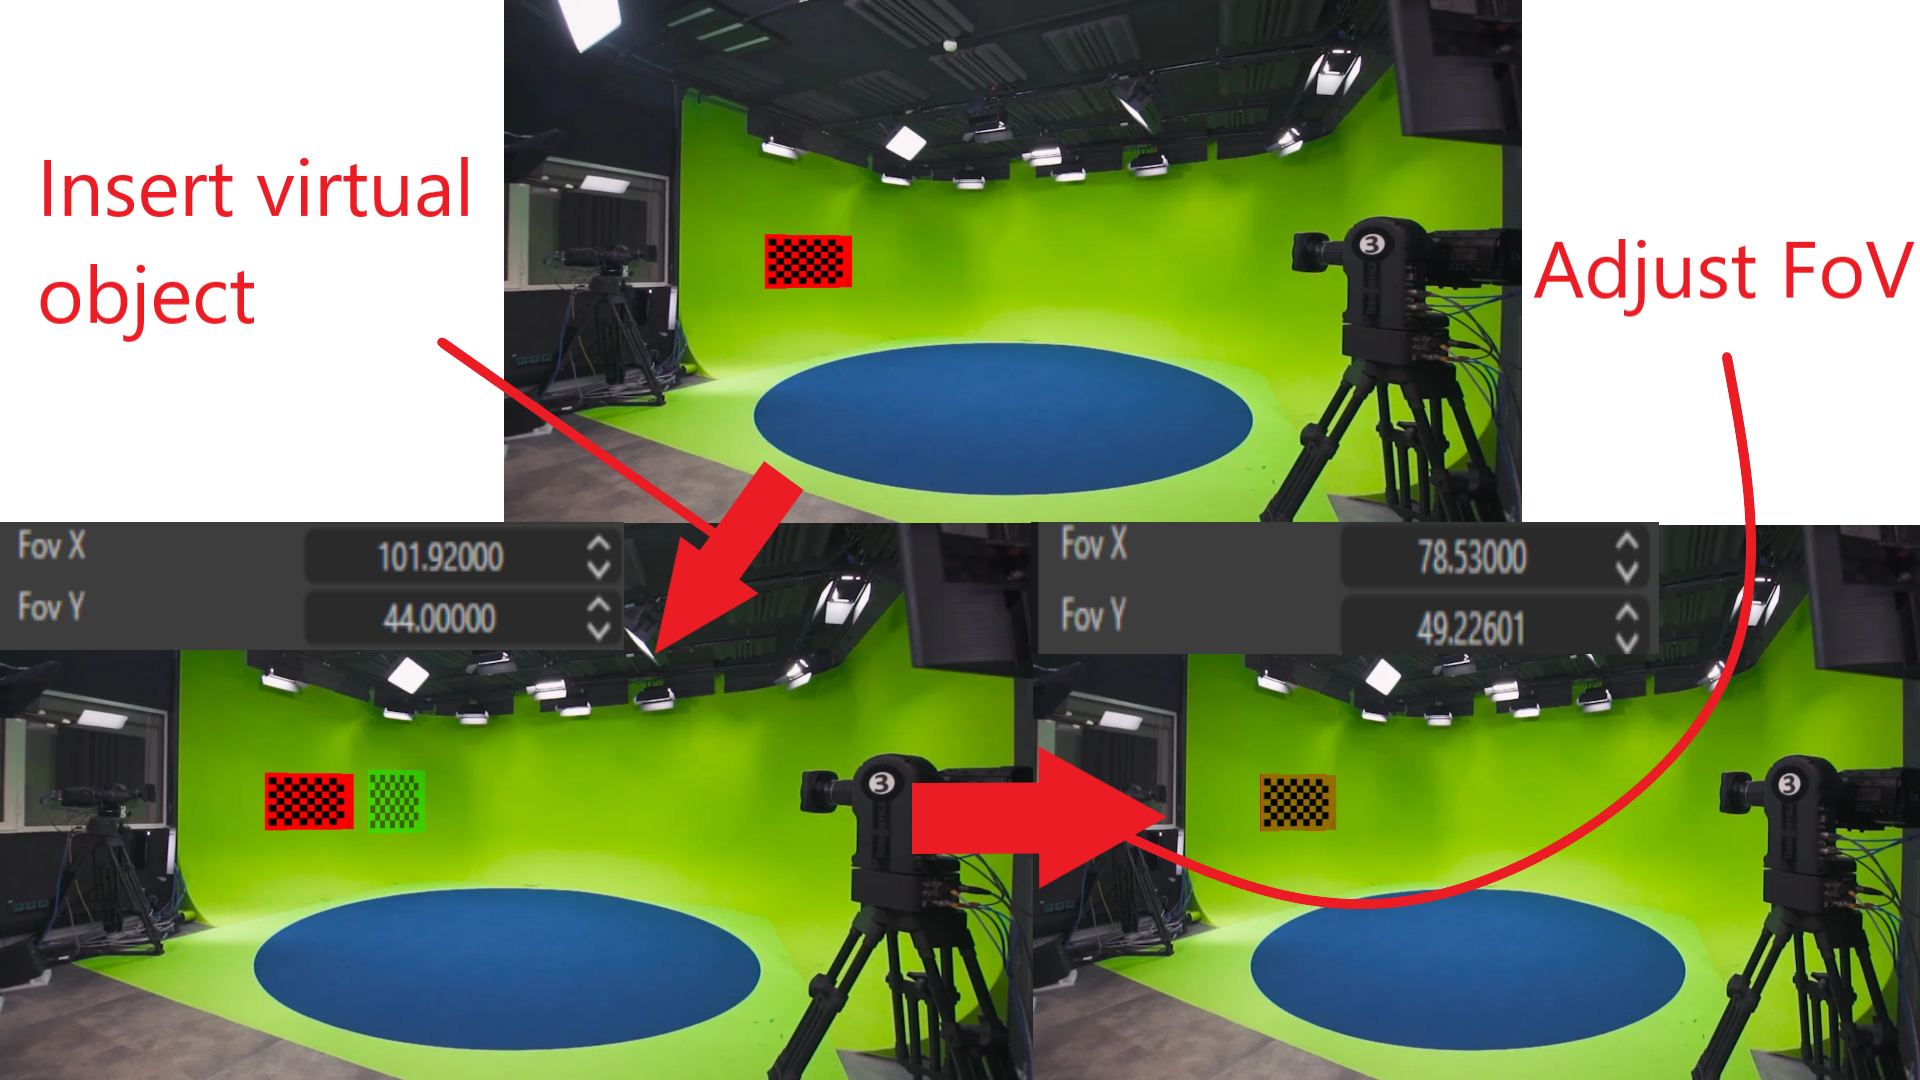
\includegraphics[width=\textwidth]{Images/01intro/FoV_procedure.png}
    \caption{FoV calibration procedure example}
    \label{fig:FoV_pro}
    \end{figure}

    \item \textbf{\( k_1 \) and \( k_2 \):} Move the object to the edges of the frame. Adjust \( k_1 \) and \( k_2 \) coefficients until alignment is achieved. Repeat across all zoom levels. Figure \ref{fig:K1_pro} illustrates the K1 calibration. The K2 calibration is analog to the K1 calibration, however the real object should be moved to the corner of the image. Figure \ref{fig:CP} illustrates where the object needs to be for each specific coefficient calibration.

    \begin{figure}[h]
    \centering
    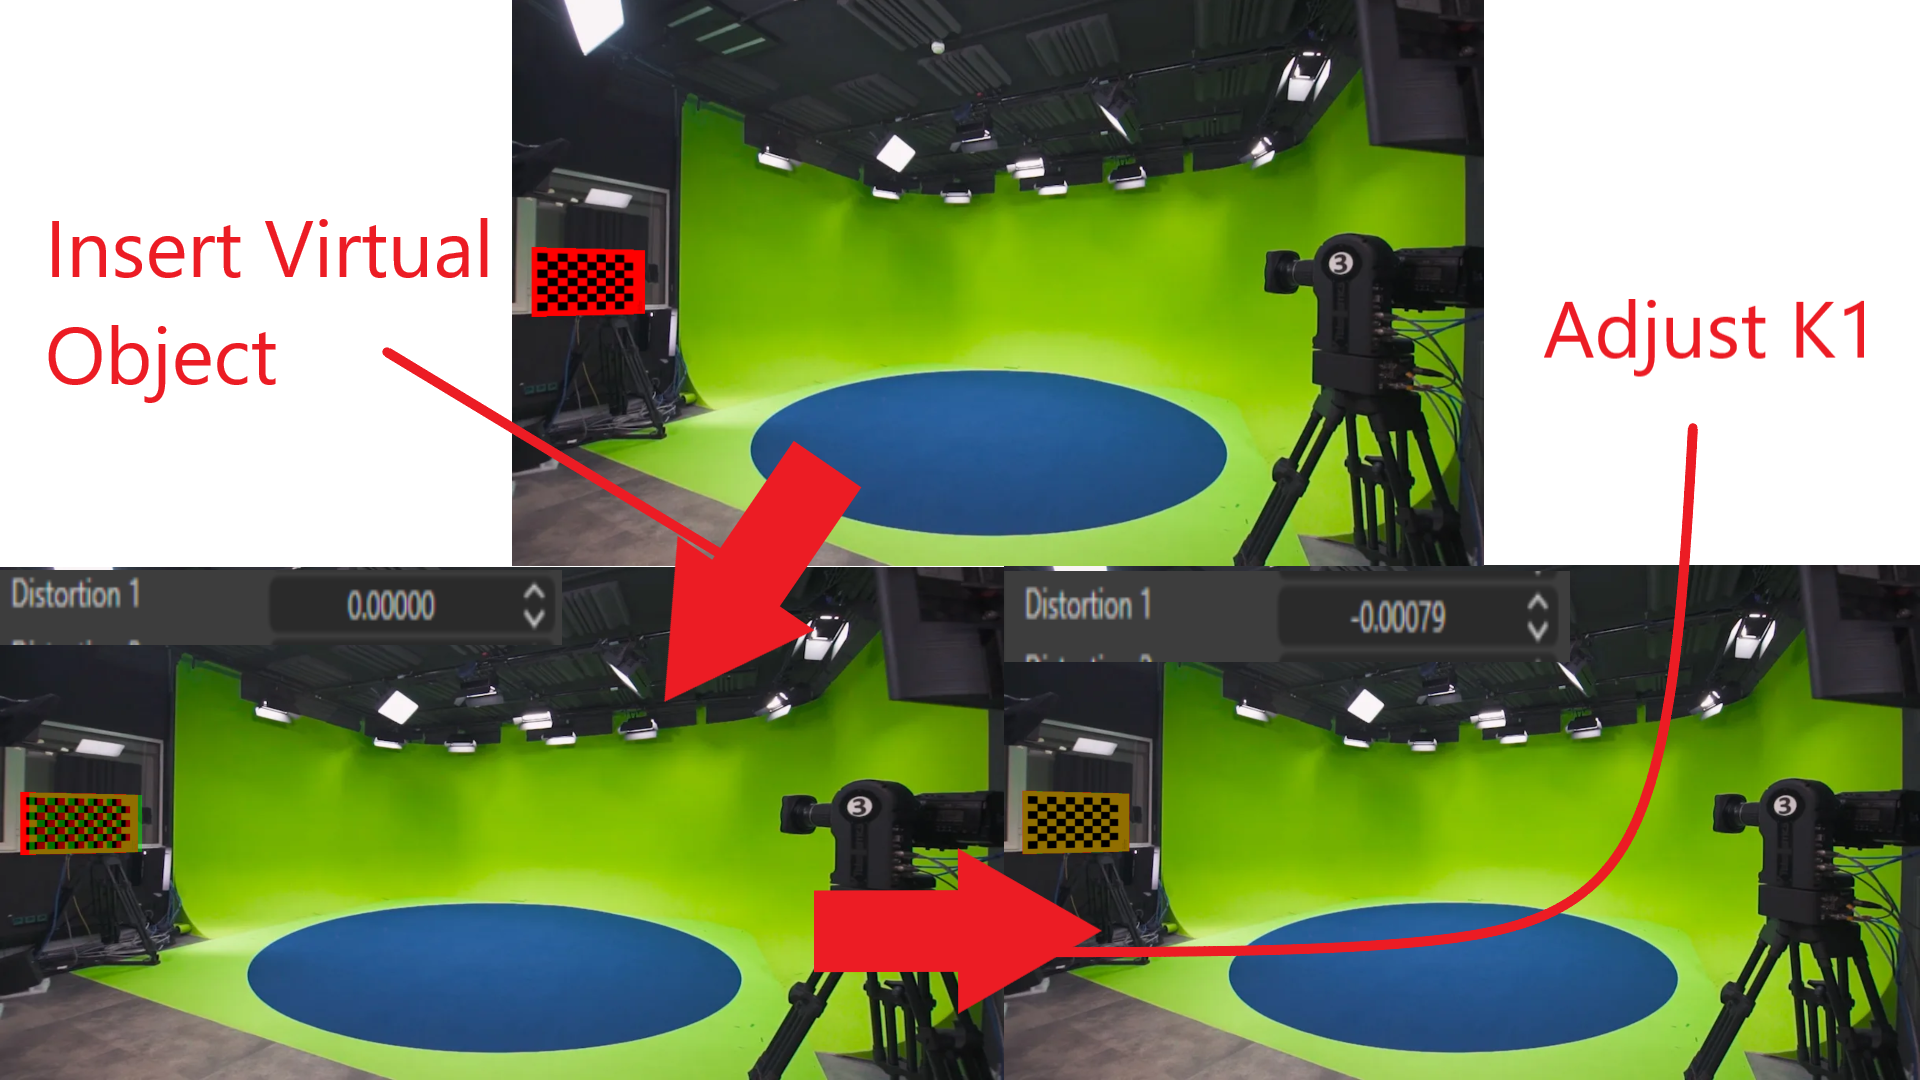
\includegraphics[width=\textwidth]{Images/01intro/K1_pro.png}
    \caption{K1 calibration procedure example}
    \label{fig:K1_pro}
    \end{figure}
    
    \item \textbf{Nodal Point:} Follow the steps to align two reference objects at different depths, ensuring there is \textbf{no parallax effect}\footnote{The \textbf{no parallax effect} occurs when a camera rotates around its \textit{nodal point}, preventing any apparent shift between foreground and background objects. This ensures that elements at different depths remain perfectly aligned, eliminating unwanted distortions caused by parallax. Achieving this effect is crucial for seamless panoramic photography and precise image stitching, as it allows multiple frames to blend naturally without misalignment.} when the camera rotates slightly.
\end{enumerate}


\noindent Figure \ref{fig:CP} represents the location where the real object should be for each coefficient determination.

\begin{figure}
    \centering
    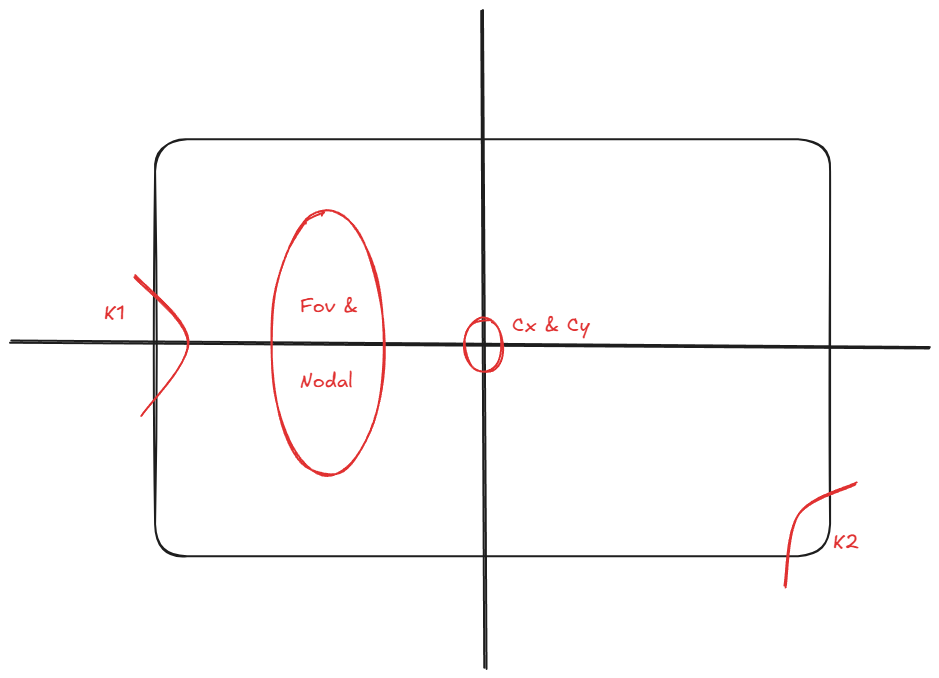
\includegraphics[width=\textwidth]{Images/02stateart/Calibration Parameters.png}
    \caption{Calibration Parameters}
    \label{fig:CP}
\end{figure}

\subsubsection*{Challenges of Current Method}

\noindent The current solution is effective, but it has limitations:

\begin{itemize}
    \item Time-intensive calibration process.
    

    \begin{table}[h]
        \centering
        \begin{tabular}{|l|c|}
            \hline
            \textbf{Coefficient} & \textbf{Calibration Time (min)} \\ \hline
            Center-shift & 5 - 10 \\ \hline
            FoV & 60 - 120 \\ \hline
            K1 & 60 - 120 \\ \hline
            K2 & 60 - 120 \\ \hline
            Nodal & 60 - 120 \\ \hline
        \end{tabular}
        \caption{Calibration Times for Each Coefficient}
        \label{tab:calibration_times}
    \end{table}

    \item Reliance on operator expertise for accurate results.
    \item Lack of automation for dynamic zoom and focus adjustments.
\end{itemize}

\subsection{Goals and Metrics}

\noindent The primary goal of this project is to improve the calibration process, making it faster, more reliable, and less dependent on the expertise of the operator. The success of this solution will be evaluated based on:

\begin{enumerate}
    \item \textbf{Accuracy of the distortion coefficients compared to manual calibration.} This accurancy will me measured by simulating images with known distortion coefficients using the $R^3$ software and comparing them to the experimental results. The goal is for each coefficient to have a relative error of less then 5\%.
    \item \textbf{Reduction in calibration time.} The goal is to reduce the calibration time to 30 minutes or less.
    \item \textbf{Consistency across multiple zoom and focus levels.} Which will be measured by analysing multiple zoom and focus levels and comparing the results.
    \item \textbf{Automation of the calibration process.} The goal is to automate the calibration process as much as possible, reducing the need for manual adjustments.
\end{enumerate}

\section{Document Overview}\label{sec:doc_overview}
